%% =====================================================================
%%  logbook_common.tex  -  cấu hình DÙNG CHUNG cho Logbook1.tex & Logbook2.tex
%%  (bố cục lấy từ main.tex / Book.cls của giảng viên: cover, mục lục,
%%   trang tiêu đề "LOGBOOK n", chân trang "Page n" + đường kẻ)
%%
%%  Biên dịch bằng LuaLaTeX (khuyến nghị, đã kiểm tra):
%%      lualatex Logbook1.tex   (chạy 2 lần để có mục lục)
%%      hoặc: latexmk Logbook1.tex   (đã có sẵn file latexmkrc)
%% =====================================================================

% --- fontspec chỉ để gõ tiếng Việt có dấu trong khối thông tin sinh viên ---
\ifdefined\directlua
  \usepackage{fontspec}          % LuaLaTeX
\else\ifdefined\XeTeXversion
  \usepackage{fontspec}          % XeLaTeX
\fi\fi

\usepackage[a4paper,tmargin=2cm,bmargin=2.5cm,lmargin=3.5cm,rmargin=2.0cm]{geometry}
\usepackage{color,calc,graphicx}
\usepackage{amsmath,amssymb,amsfonts,enumitem}
\usepackage{gensymb}
\providecommand{\micro}{\ifmmode\text{\textmu}\else\textmu\fi}   % dự phòng khi gensymb không có \micro (XeLaTeX)
\usepackage{float}
\usepackage{titlesec}
\usepackage{fancyhdr}
\usepackage{chngcntr}
\usepackage{eso-pic}
\usepackage[absolute,overlay]{textpos}
\usepackage{afterpage}

% ---------------------------------------------------------------------
%  Font chữ: Utopia thu nhỏ 0.92 (đúng tỉ lệ gói "fourier" mà mẫu dùng).
%  Tự khai báo nên cho kết quả GIỐNG NHAU trên mọi máy, không cần fourier.
% ---------------------------------------------------------------------
\usepackage[T1]{fontenc}
\makeatletter
\def\pus@decl#1#2#3#4#5{% encoding, series, shape, tfm
  \DeclareFontShape{#1}{pus}{#2}{#3}{<->s*[0.92]#4}{}}
\DeclareFontFamily{T1}{pus}{}
\pus@decl{T1}{m}{n}{putr8t}{}\pus@decl{T1}{m}{sl}{putro8t}{}\pus@decl{T1}{m}{it}{putri8t}{}
\pus@decl{T1}{m}{sc}{putrc8t}{}
\pus@decl{T1}{b}{n}{putb8t}{}\pus@decl{T1}{b}{sl}{putbo8t}{}\pus@decl{T1}{b}{it}{putbi8t}{}
\DeclareFontShape{T1}{pus}{bx}{n}{<->ssub * pus/b/n}{}
\DeclareFontShape{T1}{pus}{bx}{sl}{<->ssub * pus/b/sl}{}
\DeclareFontShape{T1}{pus}{bx}{it}{<->ssub * pus/b/it}{}
\DeclareFontFamily{TS1}{pus}{}
\pus@decl{TS1}{m}{n}{putr8c}{}\pus@decl{TS1}{m}{sl}{putro8c}{}\pus@decl{TS1}{m}{it}{putri8c}{}
\pus@decl{TS1}{b}{n}{putb8c}{}\pus@decl{TS1}{b}{sl}{putbo8c}{}\pus@decl{TS1}{b}{it}{putbi8c}{}
\DeclareFontShape{TS1}{pus}{bx}{n}{<->ssub * pus/b/n}{}
\DeclareFontShape{TS1}{pus}{bx}{sl}{<->ssub * pus/b/sl}{}
\DeclareFontShape{TS1}{pus}{bx}{it}{<->ssub * pus/b/it}{}
\DeclareFontFamily{OT1}{pus}{}
\pus@decl{OT1}{m}{n}{putr7t}{}\pus@decl{OT1}{m}{sl}{putro7t}{}\pus@decl{OT1}{m}{it}{putri7t}{}
\pus@decl{OT1}{b}{n}{putb7t}{}\pus@decl{OT1}{b}{sl}{putbo7t}{}\pus@decl{OT1}{b}{it}{putbi7t}{}
\DeclareFontShape{OT1}{pus}{bx}{n}{<->ssub * pus/b/n}{}
\DeclareFontShape{OT1}{pus}{bx}{sl}{<->ssub * pus/b/sl}{}
\DeclareFontShape{OT1}{pus}{bx}{it}{<->ssub * pus/b/it}{}
\makeatother
\renewcommand{\rmdefault}{pus}
\renewcommand{\familydefault}{\rmdefault}
\usepackage[italic]{mathastext}   % chữ cái trong công thức dùng cùng font Utopia

% ---------------------------------------------------------------------
%  Tiếng Việt cho khối thông tin sinh viên (Họ và tên / MSSV / Nhóm)
% ---------------------------------------------------------------------
\ifdefined\directlua
  \newfontfamily\vnfont{Latin Modern Roman}
\else\ifdefined\XeTeXversion
  \newfontfamily\vnfont{Latin Modern Roman}
\else
  % pdfLaTeX (chưa kiểm tra được trong môi trường này): dùng mã hoá T5
  \usepackage[utf8]{inputenc}
  \usepackage[T5,T1]{fontenc}
  \newcommand{\vnfont}{\fontencoding{T5}\fontfamily{cmr}\selectfont}
\fi\fi

\usepackage{hyperref}
\hypersetup{
  colorlinks=true,
  linkcolor=black,
  filecolor=magenta,
  urlcolor=blue,
}

% ---------------------------------------------------------------------
%  Chân trang (đúng như mẫu)
% ---------------------------------------------------------------------
\pagestyle{fancy}
\lhead[]{}\chead[]{}\rhead[]{}
\lfoot[\sl Page \thepage]{\it Electronic Device Component \hfil}
\cfoot[]{}
\rfoot[\it HCMUT - Computer Engineering]{\sl Page \thepage}
\renewcommand{\headrulewidth}{0pt}
\renewcommand{\footrulewidth}{1pt}
\setlength{\parindent}{0pt}

\newcommand\blankpage{%
    \null
    \thispagestyle{empty}%
    \addtocounter{page}{0}%
    \newpage}

% ---------------------------------------------------------------------
%  Tiêu đề chương: "LOGBOOK n"
% ---------------------------------------------------------------------
\renewcommand{\chaptername}{Logbook}
\titleformat{\chapter}[display]
  {\bfseries\huge}
  {\filright\MakeUppercase{\chaptertitlename} \huge\thechapter}
  {21.8pt}
  {\titlerule\vspace{11.05pt}\filleft}
  [\vspace{10.85pt}\titlerule]
\titlespacing*{\chapter}{0pt}{50.1pt}{40pt}

\counterwithin*{section}{chapter}
\counterwithin*{subsection}{section}
\counterwithin*{subsubsection}{subsection}
\newcommand{\answer}{}   % (giữ cho tương thích với \def\answer{1} trong nội dung)

% ---------------------------------------------------------------------
%  Thông tin sinh viên in trên trang tiêu đề của logbook
%  (đặt theo toạ độ tuyệt đối, khớp vị trí bảng "Full name / Student ID / Group" của mẫu)
% ---------------------------------------------------------------------
\providecommand{\Nhom}{\hbox to 2.5cm{\dotfill}}   % nếu chưa khai báo nhóm -> để trống kẻ chấm
\providecommand{\ThanhVien}{Họ và tên & MSSV\\}         % mỗi dòng:  Họ tên & MSSV \\
\newcommand{\logbookinfo}{%
  {\vnfont\fontsize{15.9}{19}\selectfont
   \renewcommand{\arraystretch}{1.157}%
   \begin{tabular}[t]{@{}p{6.6cm}@{}l@{}}
     {\bfseries Họ và tên:} & {\bfseries MSSV:}\\[3.8pt]
     \ThanhVien
     \multicolumn{2}{@{}l}{{\bfseries Nhóm:}\ \Nhom}
   \end{tabular}}}

\renewcommand{\chap}[1]{%
    \chapter{#1}
    \thispagestyle{empty}
    \AddToShipoutPictureBG*{
\includegraphics[width=\paperwidth,height=\paperheight]{source/picture/chapter.png}}
    \AddToShipoutPictureFG*{\put(190.9,469.1){\logbookinfo}}
    \newpage
}

% ---------------------------------------------------------------------
%  \MakeLogbook{số logbook}{file nội dung}
%  Thứ tự giống main.tex: bìa -> trang trắng -> mục lục -> chương
% ---------------------------------------------------------------------
\newcommand{\MakeLogbook}[2]{%
  \thispagestyle{empty}
  \AddToShipoutPictureBG*{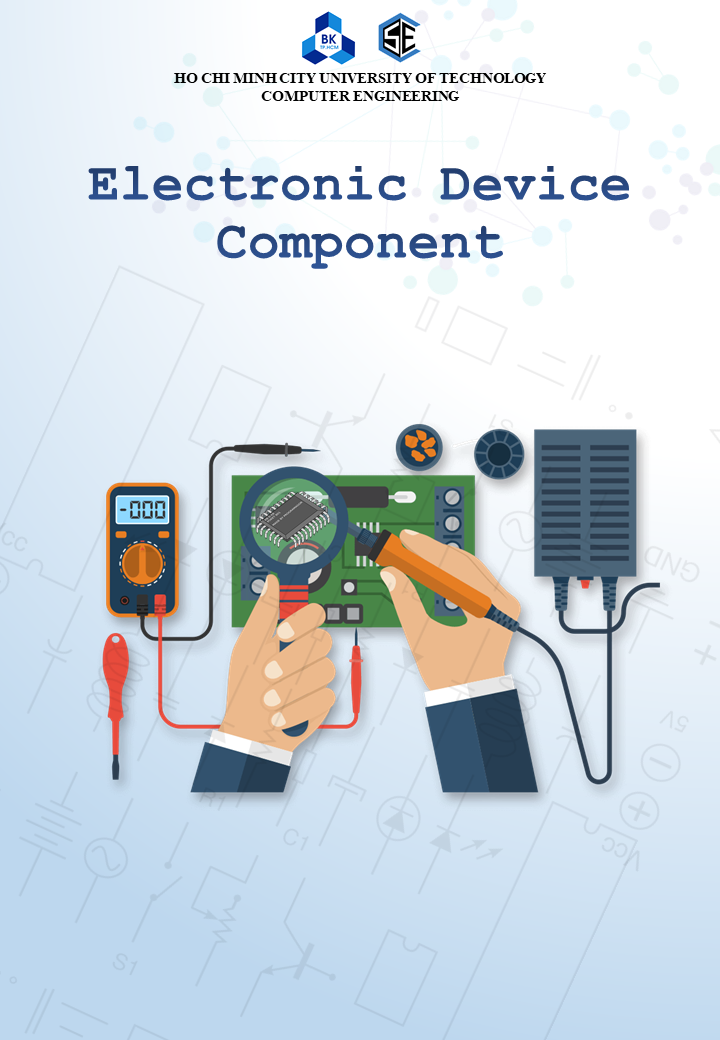
\includegraphics[width=\paperwidth,height=\paperheight]{source/picture/cover.png}}
  \begin{textblock*}{22cm}(0cm,27cm)
    \begin{center}
      \textbf{Dr. Le Trong Nhan}
    \end{center}
  \end{textblock*}
  \begin{center}\bf{\Large }\end{center}
  \afterpage{\blankpage}
  \tableofcontents
  \setcounter{chapter}{\numexpr#1-1\relax}
  \input{#2}
}
